\section{Polsby-Popper}\label{sec:pp}

The first compactness score we analyze is the \textit{Polsby-Popper
score}, which takes the form of an \textit{isoperimetric quotient},
meaning it measures how much area a region's perimeter encloses,
relative to all other regions with the same perimeter.
\mute{
\begin{definition}\label{def:pp}
  The Polsby-Popper score of a region $\Omega$ is defined to be
  $$\mathrm{PP}(\Omega) = \frac{4\pi
  \cdot\mathrm{area}(\Omega)}{\mathrm{perim}(\Omega)^2}$$ 
  and takes the form of an \textit{isoperimetric quotient} \abn{what's
  an isoperimetric quotient?}.  
\end{definition}
It's easy to check that among all regions in the plane with a fixed
area, a circle of that area has the shortest perimeter, and
equivalently, the Polsby-Popper score for a circle is 1.  We can
analogously define the score on the sphere by transferring this
intuition of isoperimetry.  In this first attempt, we transfer this
notion directly to the sphere, and define the Polsby-Popper score on
the sphere to be exactly the function in Definition~\ref{def:pp}.
}
\abn{Rewrote Polsby-Popper intro to be more formulas and less
words}\zs{looks good. leaving the comment here so we know something
changed.}
\begin{definition}\label{def:pp}
  The Polsby-Popper score of a region $\Omega$ is defined to be
  $$\mathrm{PP}_X(\Omega) = \frac{4\pi
  \cdot\mathrm{area}_X(\Omega)}{\mathrm{perim}_X(\Omega)^2}$$ 
  Where $X$ is either the sphere $S$ or the plane $\R^2$, and
  $\mathrm{area}_X$ and $\mathrm{perim}_X$ are the area and perimeter
  respectively of $A$ in $X$.
\end{definition}
The ancient Greeks were first to observed that if $\Omega$ is a region
in the plane, then $4\pi\cdot\mathrm{area}(\Omega)\leq
\mathrm{perim}(\Omega)^2$, with equality if and only if $\Omega$ is
a circle. This seemingly obvious fact took a long time to prove%
\abn{TODO: find a good reference on the history of the isoperimetric
ratio}, and became known as the \textit{isoperimetric inequality} in
the plane.  This means that $0\le \mathrm{PP}_{\R^2}(\Omega)\le 1$,
where the Polsby-Popper score is equal to $1$ only in the case of
a circle. In particular, the Polsby-Popper score is scale-invariant in
the plane. An isoperimetric inequality for the sphere exists, and we
state it as the following lemma.  For a more detailed treatment of
isoperimetry in general, see \cite{osserman1979bonnesen}, and for
a proof of this inequality for the sphere, see \cite{rado}.
\zs{rewrote slightly}
\begin{lemma}
  If $\Omega$ is a region on the \mute{half-sphere} sphere with area
  $A$ and perimeter $P$, then $P^2\geq A^2-4\pi A$ with equality if
  and only if $\Omega$ is a spherical cap.
\end{lemma}
A consequence of this is that among all regions on the sphere with
a fixed area $A$, a spherical cap with area $A$ has the shortest
perimeter. However, the key difference between the isoperimetric 
quotient in the plane and on the sphere is that on the 
sphere, there is no scale invariance.
%\lsn{ It feels weird to  me to call this theorem a "lemma"}
%\zs{I stated it as a lemma because I don't think we need to or even
%should be proving isoperimetric inequalities in here.  We can talk
%a little more about the audience, but it's one of those things that's
%intuitively true, but in order to get a rigorous proof, you need
%a few pages of symbol chasing and worrying about edge cases.  Maybe
%we can put a proof in an appendix if we feel like we need to include
%it?}

\begin{lemma}\label{lem:ppscale}
  Let $S$ be the unit sphere, and let $\kappa(h)$ be the cap at height
  $h$ (i.e. the region comprised of all points whose $z$-coordinate is
  greater than $1-h$, where we imagine the sphere as being embedded in
  $\R^3$, centered at the origin) Then $\mathrm{PP}(\kappa(h))$ is
  a monotonically increasing function of $h$.
\end{lemma}
\zs{$A$ was a little overloaded, so I changed it to $\kappa$ \smiley{}}
\begin{figure}
  \centering
  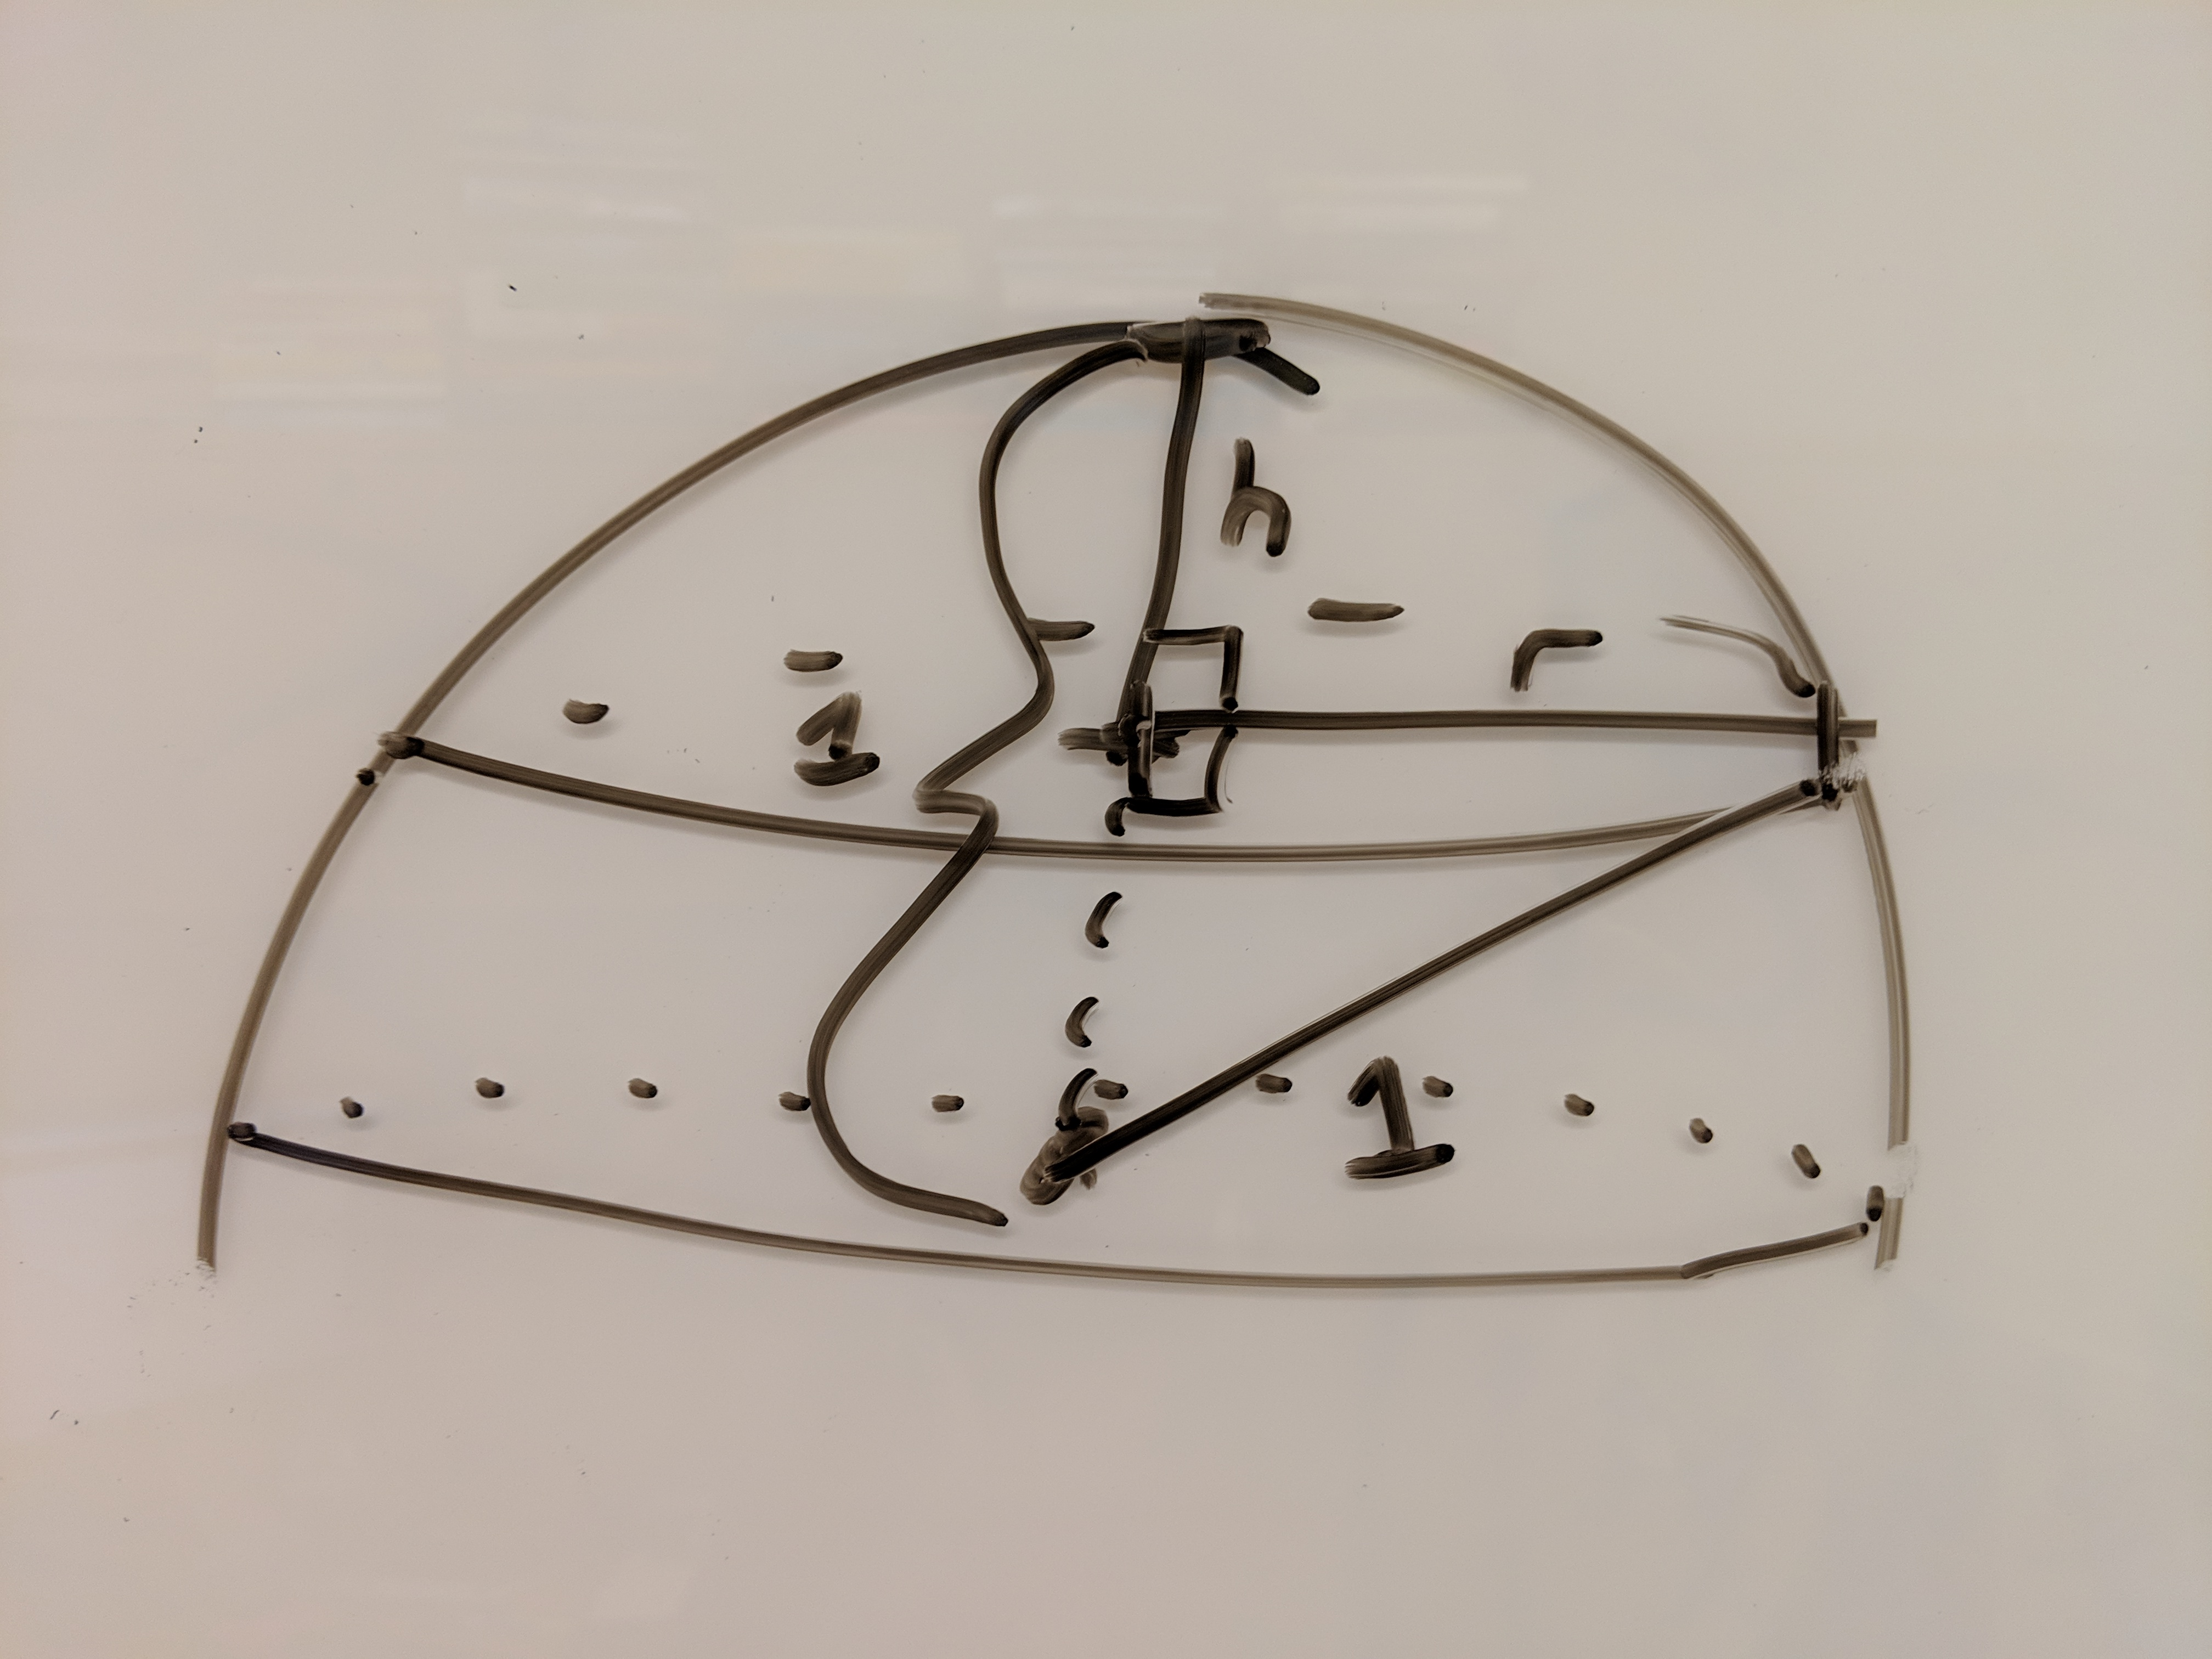
\includegraphics[width=.5\textwidth]{figs/spherical_cap.jpg}\\[1.5em]
  \caption{ The height and radius of a spherical cap. }
  \label{fig:caphr}
\end{figure}

\begin{proof}
  Let $r(h)$ be the radius of the circle bounding $\kappa(h)$. We
  compute: 
  \begin{align*}
    1 &= r(h)^2 + (1-h)^2 \text {, by right triangle trigonometry}\\ 
      &= r(h)^2 + 1 - 2h+h^2
  \end{align*}
  Rearranging, we get that $r(h)^2= 2h-h^2$, which we can plug in to
  the standard formula for perimeter:
  \begin{align*}
    \mathrm{perim}_S(\kappa(h)) = 2\pi r(h) = 2\pi \sqrt{2h-h^2}
  \end{align*}
  We can now use the Archimedian equal-area projection 
  defined by $(x,y,z) \to
  \left(\frac{x}{\sqrt{x^2+y^2}},\frac{y}{\sqrt{x^2+y^2}}, z\right)$ 
  to compute $\mathrm{area}_S(\kappa(h)) = 2\pi h$ and plug it in to 
  get:
  \zs{i think there's a better explanation than just asserting the
  existence of a projection that does this.  What about `Archimedes
  showed that the lateral surface area of a cylinder with radius $1$
  and height $2$ is the same as the surface area of the spher, and
  that the lateral projection (do figure) from the sphere onto the
  cylinder preserves area.  Using this, we have that the area of
  a spherical cap at height $h$ is'}
  \abn{I wrote something shorter and possibly more useful}
  \begin{align*}
    \mathrm{PP}_S(\kappa(h)) = \frac{4\pi (2\pi h) }{4 \pi^2 (2h-h^2)}
    = \frac{2}{2-h}
  \end{align*}
  Which is a monotonically increasing function of $h$.
\end{proof}
\begin{corollary}\label{cor:capscale}
  On the sphere, Polsby-Popper scores of caps are monotonically
  increasing with area
\end{corollary}
Using this, we can show the main theorem of this section, that no map
projection from the half-sphere to the plane can preserve the ordering
of Polsby-Popper scores for all regions.  

%\lsn{I think this is not the right statement / proof. See my email.}

\begin{theorem}\label{thm:dpp}
  If $\varphi$ is a map projection from the half-sphere to the plane,
  then there are two regions $A$ and $C$ in the half sphere such that
  the Polsby-Popper score of $C$ is greater than that of $A$ in the
  sphere, but the Polsby-Popper score of $\varphi(A)$ is greater than
  that of $\varphi(C)$ in the plane.
\end{theorem}
\begin{figure}\label{fig:dpp}
  \centering
  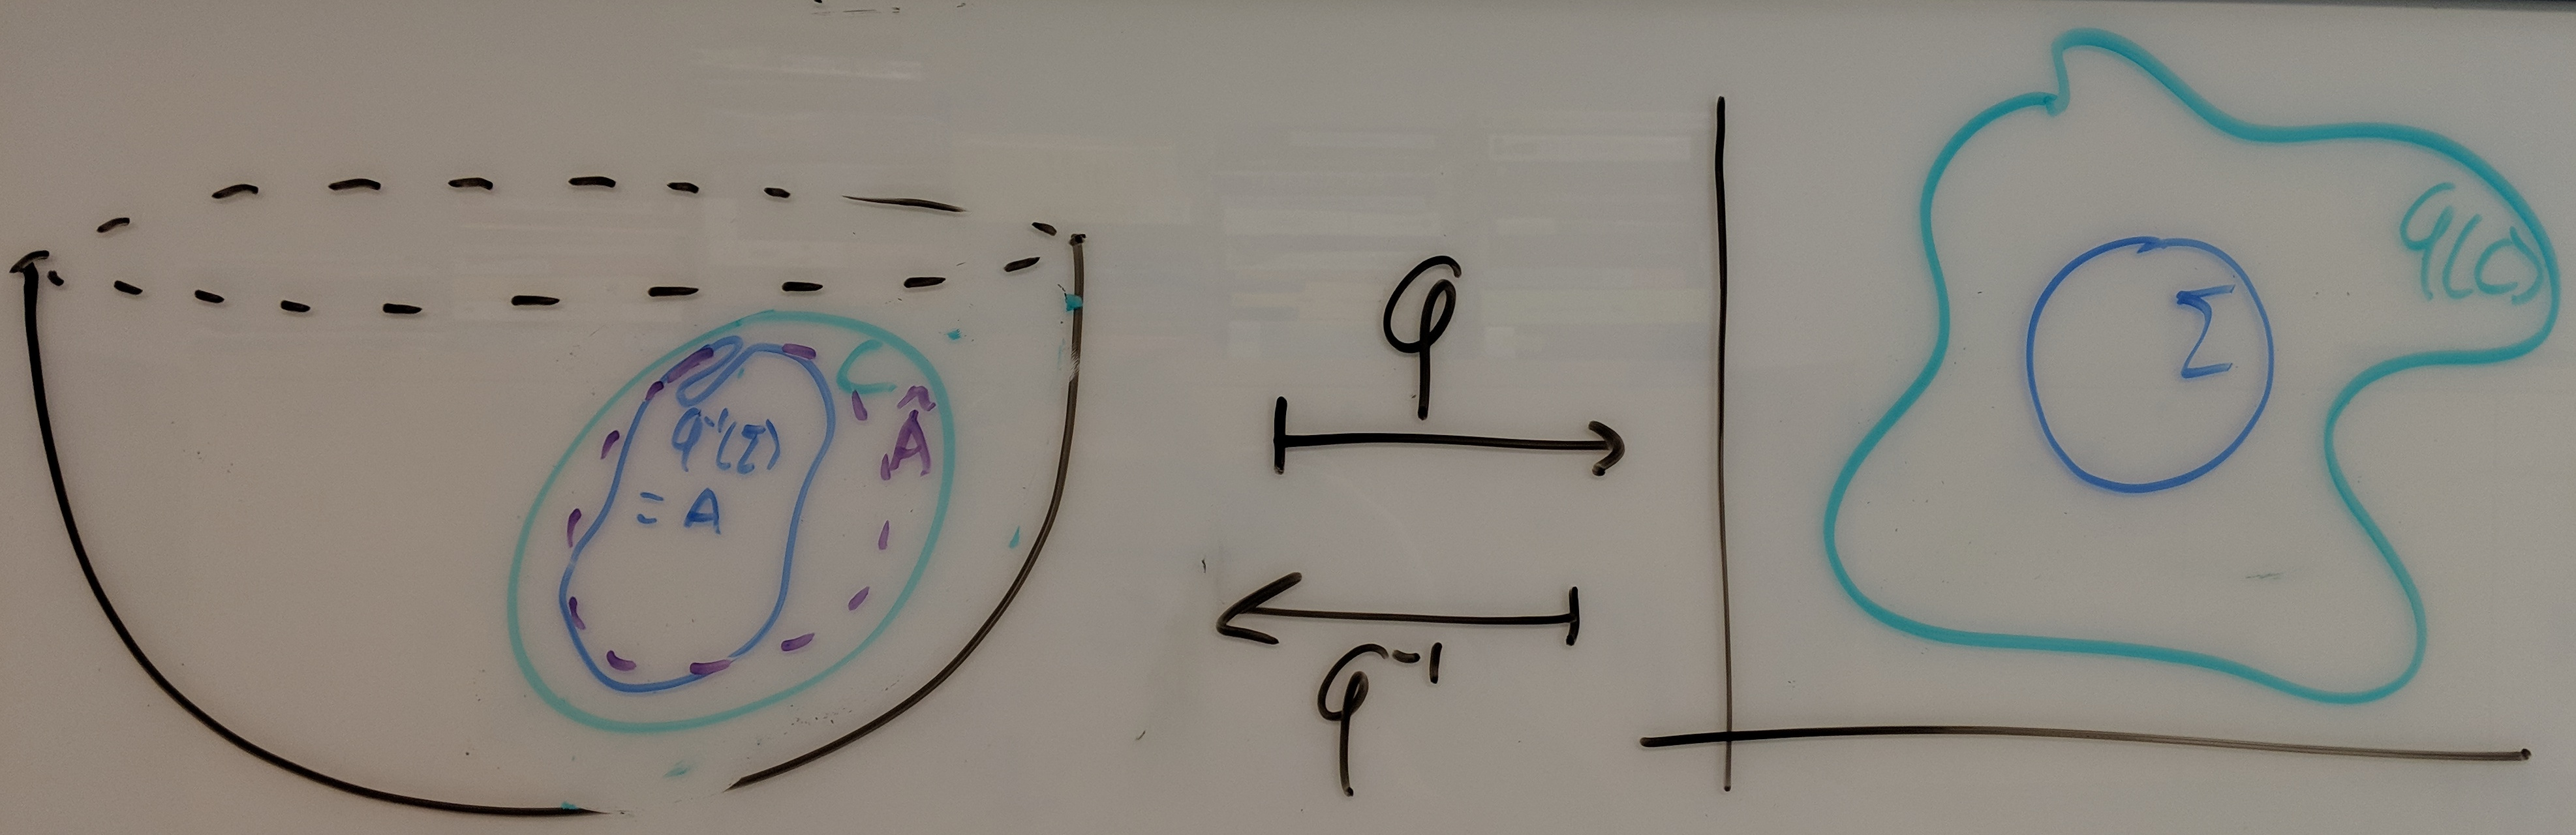
\includegraphics[width=.9\textwidth]{figs/dumb_pp_cropped.jpg}\\[1.5em]
  \caption{ The construction of regions $A$, $C$, and $\hat{A}$ in the proof of Theorem~\ref{thm:dpp}.}
\end{figure}

\begin{proof}
  Let $\varphi$ be a map projection, and take $C$ to be a cap in the
  half-sphere. Let $\Sigma$ be a circle in the plane such that $\Sigma
  \subsetneq \varphi(C)$ and let $A=\varphi^{-1}(\Sigma)$ (see
  Figure~\ref{fig:dpp}).

  %\lsn{It doesn't depend on the preimage of $\Sigma$ not being a cap,
  %because the preimage of $\Sigma$ has less area thatn $C$, so it's
  %polsby popper score will be strictly worse.  I think this
  %computation is necessary -- it's in the original doc. Also see my
  %email.}

  We now use the isoperimetric inequality for the sphere 
  and Corollary~\ref{cor:capscale} to claim that 
  $A$ does not maximilze Polsby-Popper score in the sphere.

  To see this, take $\hat{A}$ to be a cap in the sphere with 
  area equal to that of $A$. By the isoperimetric 
  inequality of the sphere, $\mathrm{PP}_S(\hat{A})\geq
  \mathrm{PP}_S(A)$. Since map projections preserve containment,
  $\Sigma\subsetneq \varphi(C)$ implies that $A\subsetneq C$, 
  meaning that $\mathrm{area}(\hat A) = \mathrm{area}(A)\lneq 
  \mathrm{area}(C)$. By Corollary~\ref{cor:capscale}, we know that
  $\mathrm{PP_S}(\hat{A})< \mathrm{PP_S}(C)$, and combining this with
  the earlier inequality, we get
  \begin{align*}
    \mathrm{PP_S}({A})\leq \mathrm{PP_S}(\hat{A})< \mathrm{PP_S}(C)
  \end{align*}

  \mute{
  By construction, $\mathrm{area}(\hat{A})=\mathrm{area}(A)$ but
  $\mathrm{area}(A) \lneq \mathrm{area}(C)$, so
  $\mathrm{area}(\hat{A})< \mathrm{area}(C)$, which means that
  $\hat{A}$ is a cap with height and radius strictly smaller than that
  of $C$.
  }

  Since $\Sigma = \varphi(A)$ maximizes the Polsby-Popper score in the
  plane, but $A$ does not do so in the sphere, we have shown that
  $\varphi$ does not preserve the maximal elements in the score
  ordering, and therefore it cannot preserve the ordering itself.
\end{proof}

The reason why every map projection fails to preserve the ordering of
Polsby-Popper scores is because the score itself is constructed from
the \textit{planar} notion of isoperimetry, and there is no reason to
expect this formula to move nicely back and forth between the sphere
and the plane.  This proof crucially exploits a scale invariance
present in the plane but not the sphere.  If we consider any circle in
the plane, it's Polsby-Popper score is definitionally equal to one,
but that is not true of every cap in the sphere.  This naturally
raises the question of whether being more careful, and defining
a compactness score which uses the isoperimetric quotient of the
surface the region is actually in will evade this problem.  We show
later that it does resolve the issue of scale-noninvariance, but it is
still induces an ordering which is not preserved by any map
projection.  We address this in Section~\ref{sec:isoper}, as it uses
on machinery we develop in the interceding sections.
